The diffraction condition in the case of a three-dimensional regular grating with elastic scattering~\cite{Kittel86} can be converted as follows:

    \begin{equation}
        \begin{cases}
            \cos{\theta_0}\sin{\Delta \theta}\cos{\left( \Delta \varphi - \varphi_0 \right)} - \sin{\theta_0} \left( \cos{\Delta \theta} - 1 \right) = \cfrac{h^{\prime} \lambda}{d}
            \\
            \sin{\Delta \theta} \sin{\left( \Delta \varphi - \varphi_0 \right)} = \cfrac{k^{\prime} \lambda}{d}
            \\
            \sin{\theta_0}\sin{\Delta \theta}\cos{\left( \Delta \varphi - \varphi_0 \right)} + \cos{\theta_0} \left( \cos{\Delta \theta} - 1 \right)= \cfrac{l^{\prime} \lambda}{d}
        \end{cases}
        \label{bragg_wolf_order_spherical}
    \end{equation}
    \begin{equation*}
    \end{equation*}

\noindent where $\Delta \theta,\:\Delta \varphi$ are the angles characterizing the deviation of the direction of the diffracted radiation relative to the incident one, $\theta_0,\:\varphi_0$ are the angles characterizing the rotation of the target (grid) in space , $h^\prime,\:k^\prime,\:l^\prime$ --- new Miller indices (\ref{3ddiffr:image}), $\vectbf{e}{\textrm{in}} = \vectbf{e}{z}$ is the fixed direction of the incident radiation, $d$ --- distance between clusters. Using (\ref{bragg_wolf_order_spherical}), we can obtain the angular distribution of diffracted radiation for given initial parameters $d$, $\lambda$, $\theta_0$, $\varphi_0$.

\begin{tikzfigure}
    \subcaptionbox{$xz$ projection.}{
        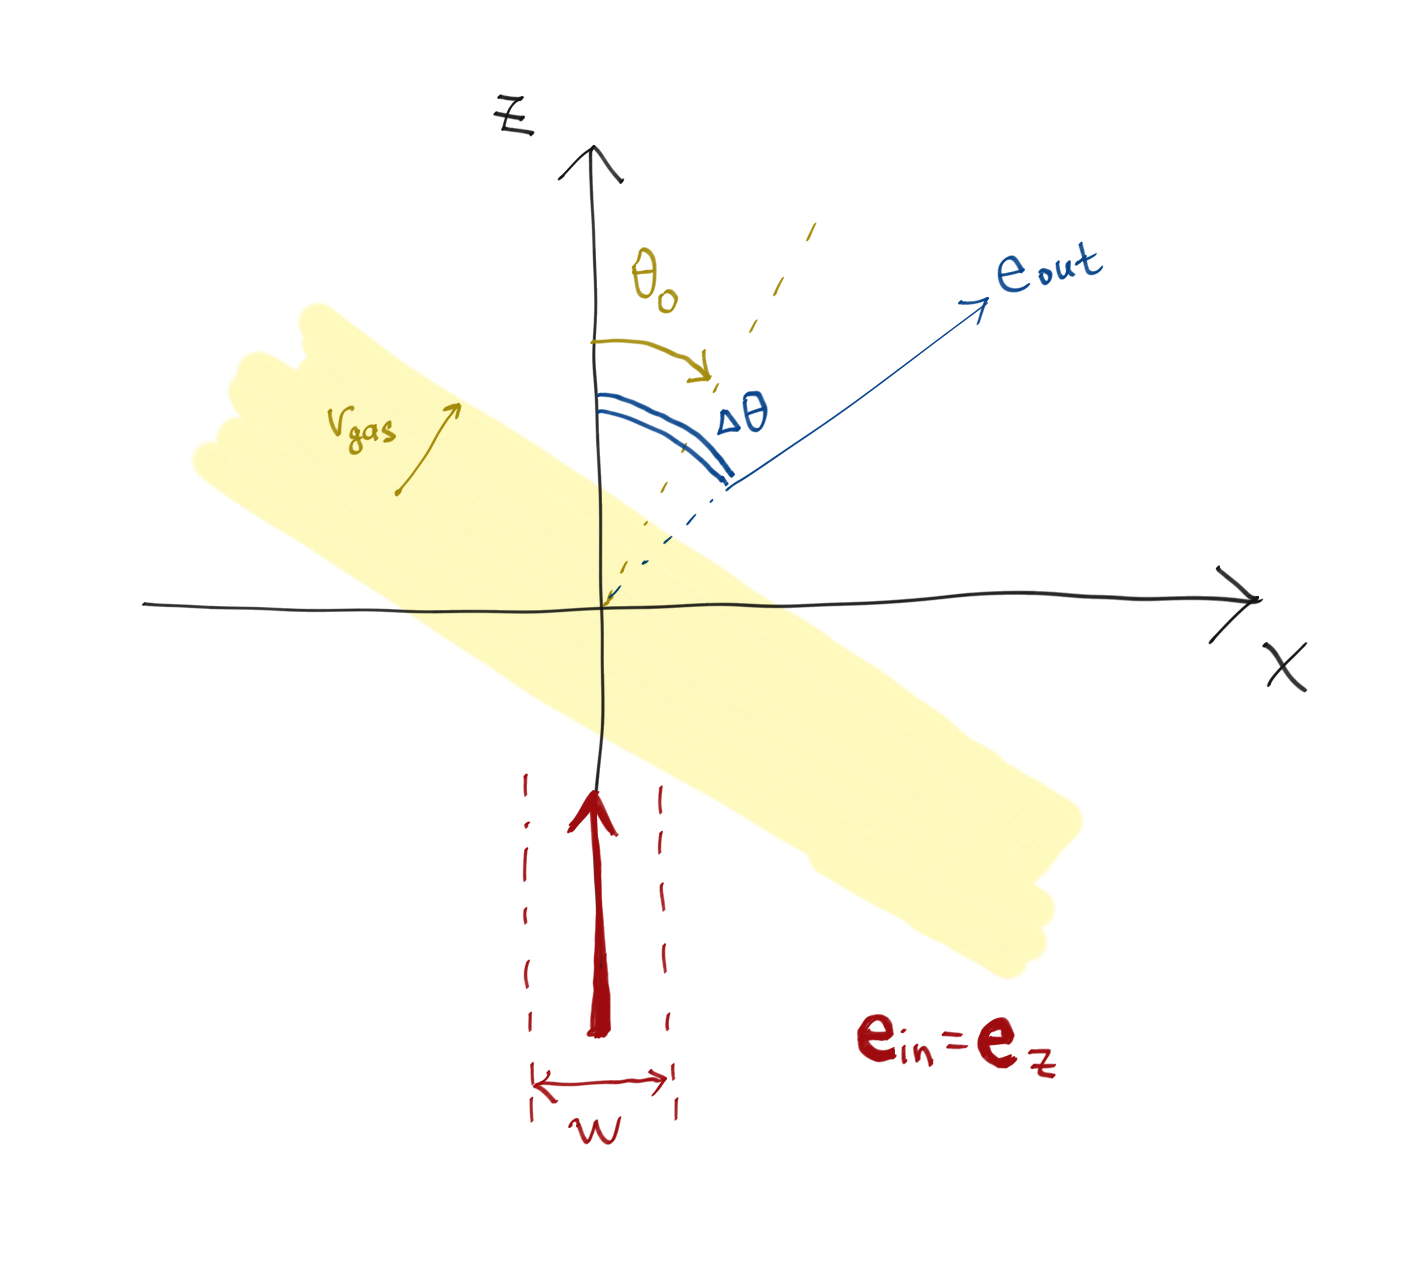
\includegraphics[width=0.43\linewidth]{../img/3ddiffrxzgas}
    }
    \hfil
    \subcaptionbox{$xy$ projection.}{
        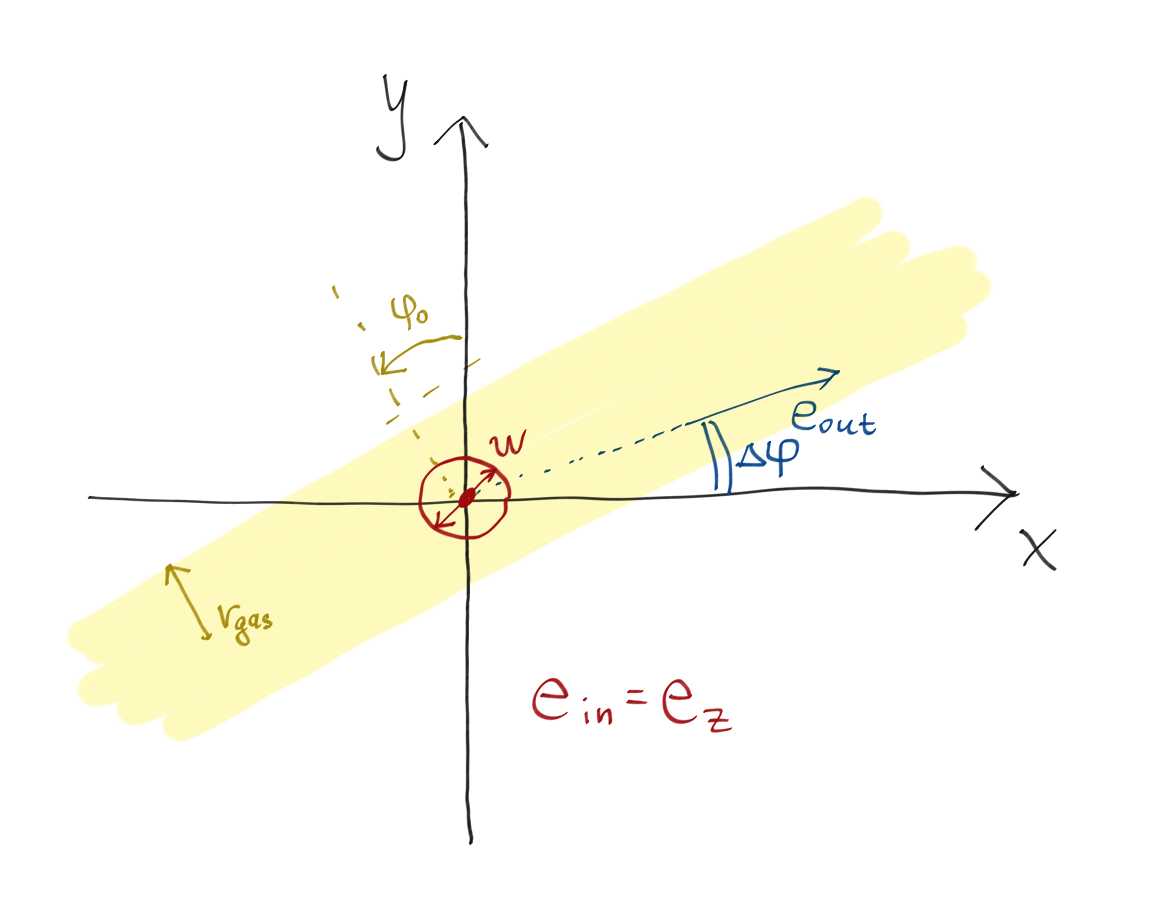
\includegraphics[width=0.43\linewidth]{../img/3ddiffrxygas}
    }
    \label{3ddiffr:image}\caption{General scheme of interaction of incident radiation with a grating. $\theta_0$, $\varphi_0$ --- characterize the target angles in space, $\Delta \theta$, $\Delta \varphi$ --- angles of deflection of the direction of the diffracted radiation relative to the incident, $r_{\textrm{gas }}$ is the radius of the gas jet representing the target, $w$ is the diameter of the Gaussian beam of incident radiation.}
\end{tikzfigure}